% Nêu tổng quan phương pháp thực hiện

\subsection{1. Thu thập và phân tích dữ liệu} 

Dữ liệu được thu thập từ nguồn công khai: một bộ dữ liệu được xây dựng bởi Chương trình Hỗ trợ Da liễu và Phẫu thuật (PAD) \cite{mahdavi2022skincancer}. Bộ dữ liệu bao gồm 2.298 mẫu từ 1.373 bệnh nhân, kết hợp giữa hình ảnh tổn thương da được chụp bằng điện thoại thông minh và tối đa 22 đặc trưng lâm sàng (tuổi, vị trí tổn thương, loại da Fitzpatrick, đường kính tổn thương, v.v.), phân thành 6 nhóm gồm 3 loại ung thư da: BCC (Basal Cell Carcinoma), MEL (Melanoma), SCC (Squamous Cell Carcinoma) và 3 loại bệnh da lành tính: ACK (Actinic Keratosis), NEV (Nevi), SEK (Seborrheic Keratosis). Quá trình tiền xử lý bao gồm chuẩn hóa và tăng cường hình ảnh da liễu (augmentation, normalization), xử lý dữ liệu lâm sàng dạng bảng (điền giá trị thiếu, mã hóa đặc trưng phân loại), cân bằng lớp do phân phối mất cân đối giữa các nhóm tổn thương, phân chia tập train/validation/test theo từng bệnh nhân để tránh data leakage, và xây dựng Feature Store để quản lý đặc trưng tập trung, đảm bảo tính nhất quán giữa môi trường huấn luyện và triển khai.
   


\subsection{2. Xây dựng mô hình} 
\subsubsection{2.1 Kiến trúc mô hình Multimodal AI: }
Mô hình được đề xuất là một hệ thống học sâu đa phương thức (Multimodal Deep Learning), được thiết kế nhằm kết hợp đồng thời hai nguồn dữ liệu dị cấu trúc: dữ liệu hình ảnh y tế (X-quang da liễu) và dữ liệu bảng thuộc tính lâm sàng (CSV). Kiến trúc tổng thể của mô hình được tổ chức theo mô hình song song hai nhánh độc lập, hội tụ tại một tầng hợp nhất đặc trưng (Late Fusion), trước khi đưa ra dự đoán phân loại cuối cùng. Cách thiết kế này cho phép mô hình khai thác tối đa thông tin từ từng phương thức riêng biệt, đồng thời tận dụng sự bổ sung lẫn nhau giữa các phương thức để nâng cao độ chính xác chẩn đoán \cite{singh_multimodal_biometrics_2024}. Quy trình hoạt động của mô hình bao gồm các giai đoạn chính sau:


   
    \paragraph{2.1.1 Giai đoạn chuẩn bị:} Giai đoạn này bao gồm ba bước chính:
    
    \begin{itemize}
    \item \textbf{Download Data (Tải dữ liệu): } Hệ thống tải xuống hai loại dữ liệu: Download Image Dataset (hình ảnh X-ray da bệnh nhân kích thước 224x224 pixels) và Download CSV dataset (dữ liệu lâm sàng chứa tuổi, giới tính, vị trí tổn thương, và các chỉ số sinh học khác)
    
    \item \textbf{Load data (Nạp dữ liệu): } Sau khi tải xuống, dữ liệu được nạp vào hệ thống thông qua hai tiến trình độc lập: Load Image Dataset và Load CSV Dataset. Bước này thực hiện việc đọc và khởi tạo các cấu trúc dữ liệu phù hợp để phục vụ quá trình tiền xử lý tiếp theo.

    \item \textbf{Preprocess data (Tiền xử lý): } Dữ liệu hình ảnh và CSV lần lượt được tiền xử lý thông qua Preprocess Image Dataset và Preprocess CSV Dataset. 

    \item \textbf{Prepare multimodal data: } Kết hợp và đồng bộ hóa hai nguồn dữ liệu, đảm bảo mỗi hình ảnh được ghép đúng với dữ liệu lâm sàng tương ứng

\end{itemize}

    \paragraph{2.1.2 Giai đoạn xây dựng mô hình:}
    Đây là giai đoạn trung tâm và phức tạp nhất của toàn bộ hệ thống, bao gồm hai nhánh xử lý song song trước khi hội tụ tại tầng Late Fusion.

    \begin{itemize}
    \item \textbf{Nhánh xử lý dữ liệu lâm sàng (CSV):} Dữ liệu đầu vào là Tabular Medical Dataset CSV chứa các trường thông tin y tế như: BG, CLASS, X, Y, RADIUS, DENSITY, BI-RADS — các chỉ số lâm sàng mô tả đặc điểm tổn thương. Chuẩn hóa (Normalization): Dữ liệu số được chuẩn hóa bằng Standard Scaler. Mạng nơ-ron Dense: Một tầng Dense với 128 → 64 neurons được sử dụng. Đầu ra: Vector đặc trưng bảng Tabular Feature Vector (64 chiều).

    
    \item \textbf{Nhánh xử lý hình ảnh X-ray:  } Dữ liệu đầu vào là các ảnh X-quang kích thước 224×224 pixel. Tiền xử lý ảnh: Bao gồm các bước resize về kích thước chuẩn, chuẩn hóa giá trị pixel, và tăng cường dữ liệu. Trích xuất đặc trưng: Mô hình ResNet50 được sử dụng làm backbone để trích xuất đặc trưng hình ảnh. Sau đó, một tầng Dense được kết nối để ánh xạ sang không gian đặc trưng chung. Đầu ra: Vector đặc trưng hình ảnh Image Feature Vector (64 chiều).


    \item \textbf{Hợp nhất và Phân loại (Fusion and Classification): } Ba vector đặc trưng 64 chiều từ ba nhánh được ghép nối (concatenate) lại thành một vector tổng hợp 192 chiều, sau đó được đưa qua: Late Fusion Layer: Dense(64) → Dense(32), thực hiện học các tương tác liên phương thức (cross-modal interactions), tích hợp thông tin từ cả ba nguồn. Lớp phân loại Softmax: Với 6 đầu ra tương ứng với 6 nhãn bệnh da liễu, lớp Softmax tính xác suất thuộc về từng nhãn: ACK, BCC, MEL, NEV, SCC, SEK.


\end{itemize}

     \paragraph{2.1.3 Giai Đoạn Đánh Giá và Dự Đoán (Prediction):}
     Sau khi huấn luyện, mô hình được đánh giá và khai thác kết quả qua bốn bước:

         \begin{itemize}
    \item \textbf{Đánh giá (Evaluate):} Mô hình được đánh giá toàn diện bằng các chỉ số: Accuracy (độ chính xác tổng thể), F1-Score (cân bằng giữa Precision và Recall), và AUC-ROC (khả năng phân biệt giữa các lớp), đặc biệt phù hợp trong bối cảnh dữ liệu y tế thường bị mất cân bằng lớp.

    
    \item \textbf{Dự đoán (Predict): } Mô hình thực hiện suy luận (inference) trên tập kiểm tra để tạo ra các dự đoán thực tế, là cơ sở để đánh giá hiệu năng thực tiễn.


    \item \textbf{Phân tích tầm quan trọng đặc trưng (Permutation Importance Analysis): } Kỹ thuật hoán vị đặc trưng được áp dụng nhằm đo lường mức độ đóng góp của từng phương thức (hình ảnh vs. bảng) vào quyết định của mô hình, cung cấp thông tin có giá trị về tính giải thích được (interpretability) của hệ thống.

   \item \textbf{Trực quan hóa (Visualization): }Ba kỹ thuật trực quan hóa được sử dụng: Grad-CAM (xác định vùng ảnh quyết định phân loại), Confusion Matrix (đánh giá phân bố lỗi theo từng lớp), và SHAP (giải thích đóng góp của từng đặc trưng bảng theo từng dự đoán cụ thể).


\end{itemize}

    \begin{figure}[!h]
    \centering
    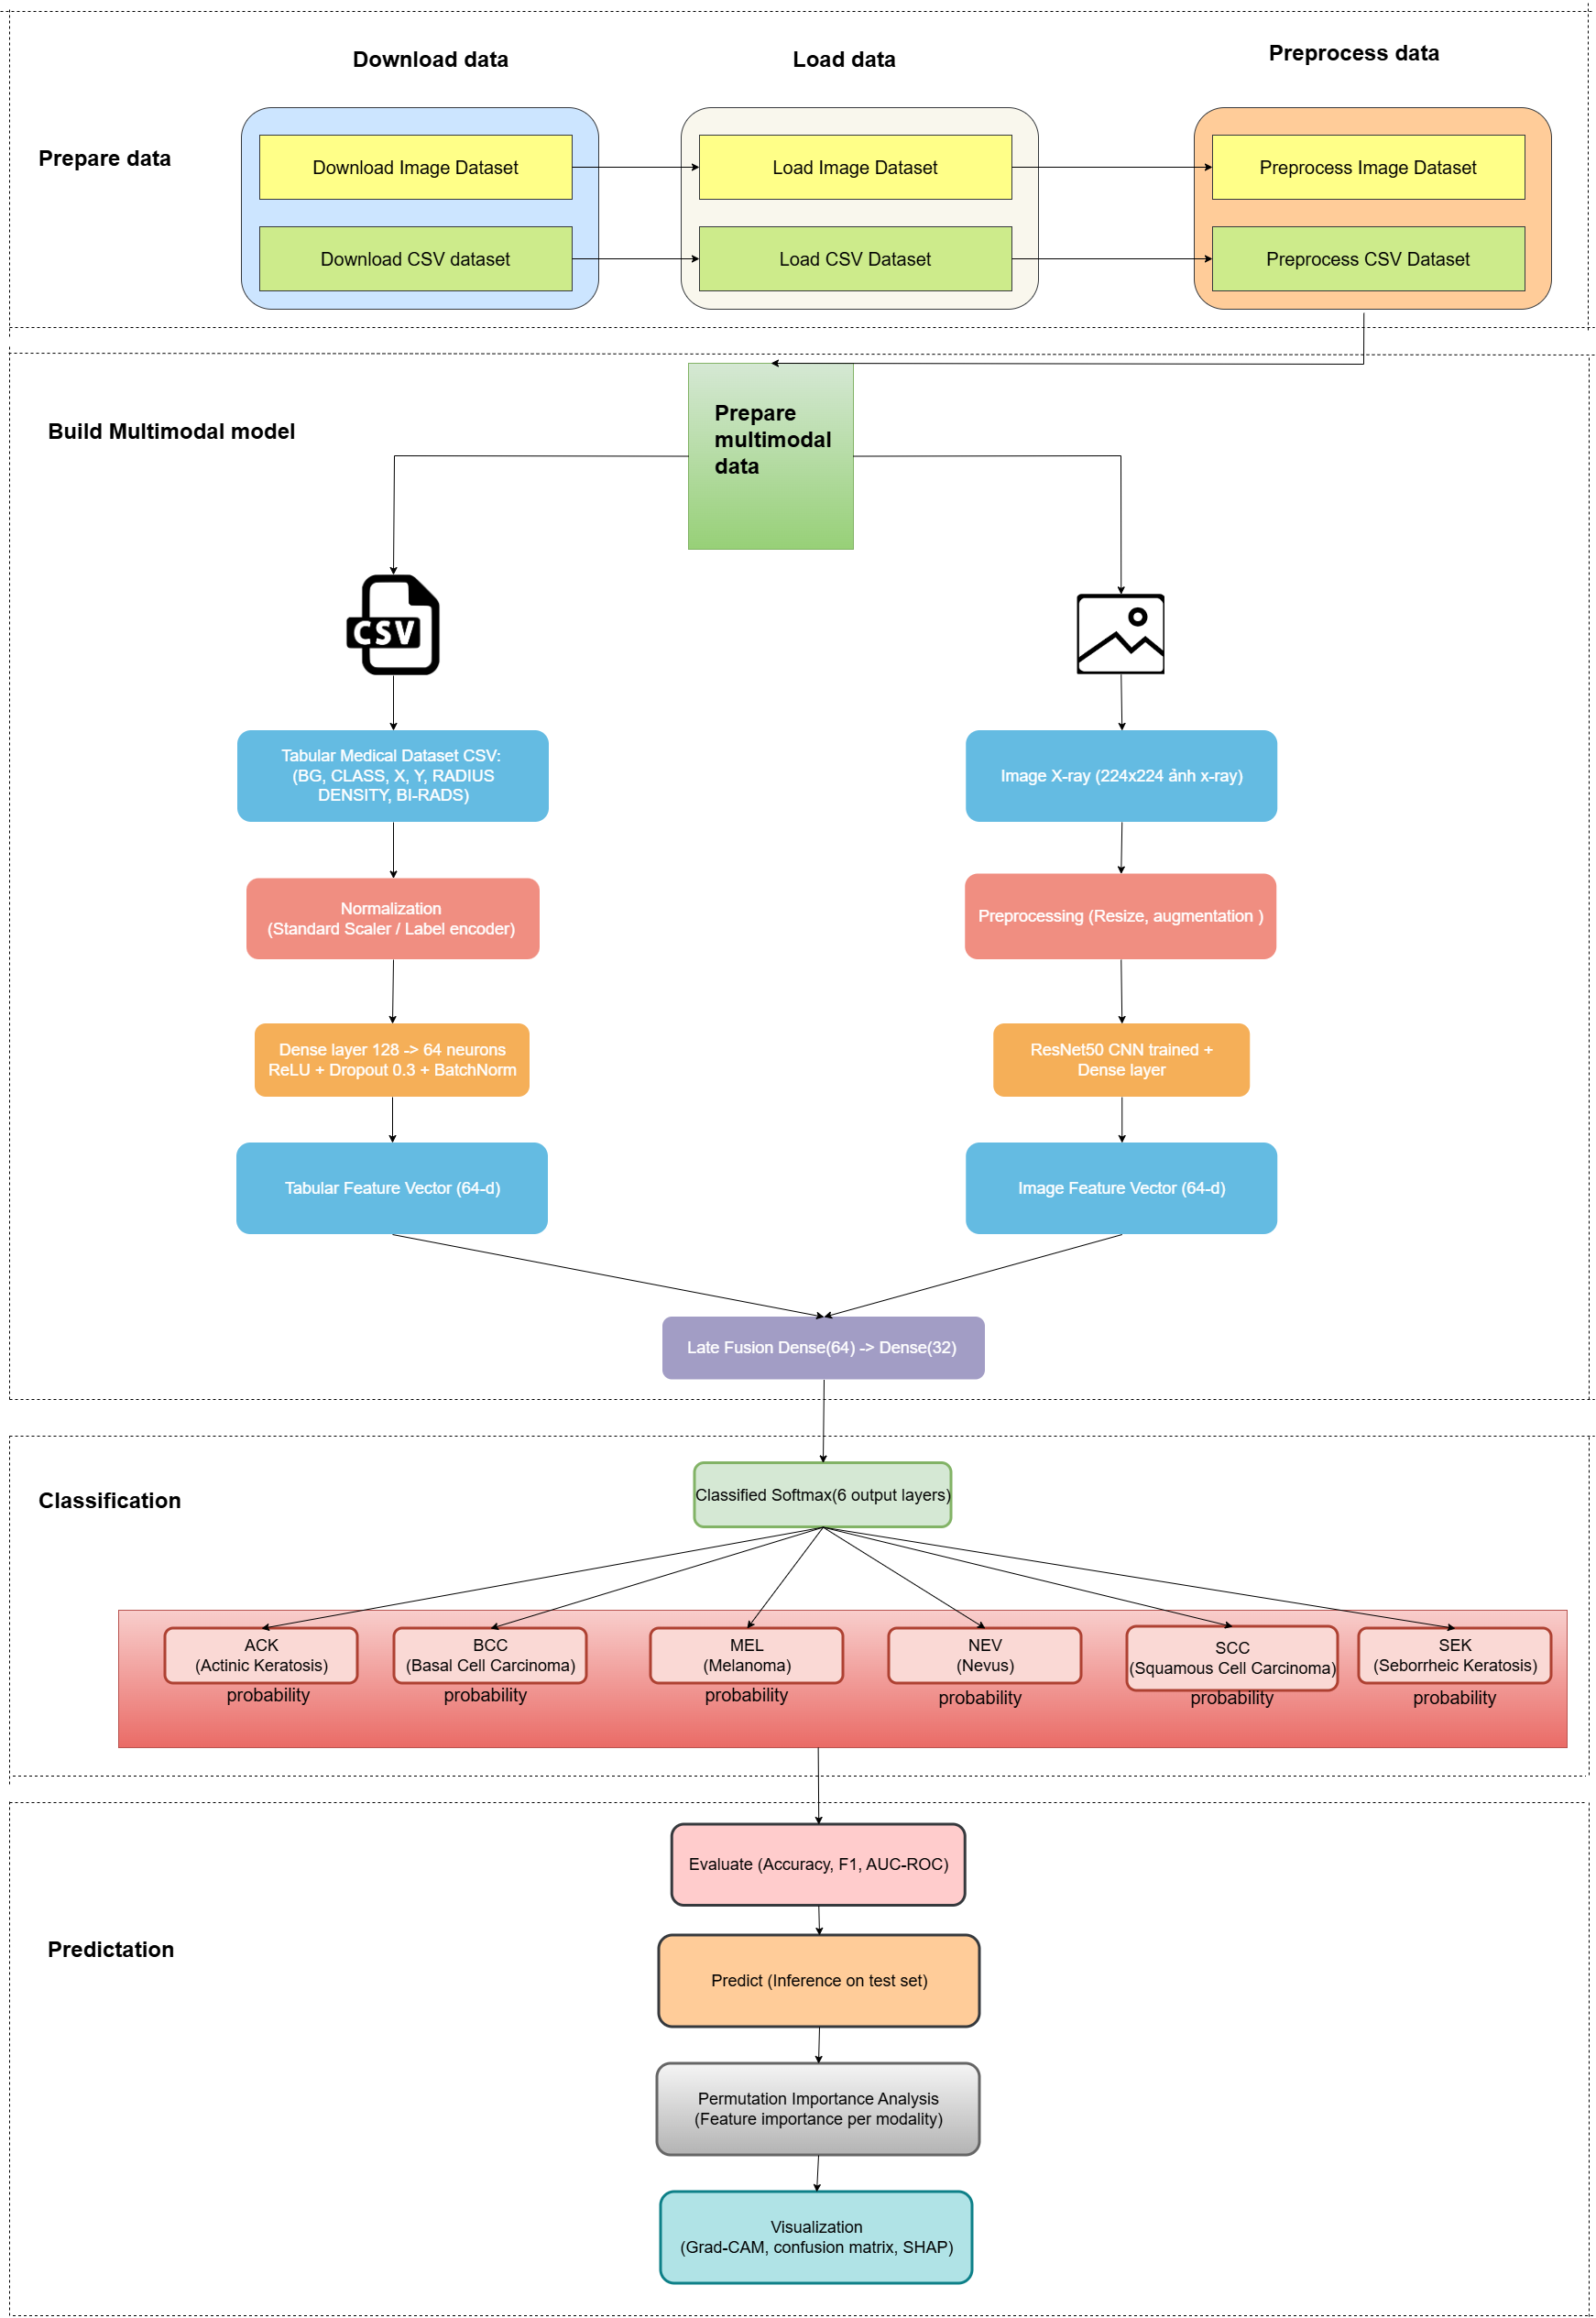
\includegraphics[width=0.95\linewidth]{Figures/KLTNmultimodal.png}
    \caption{Kiến trúc và quy trình hoạt động của mô hình Multimodal AI}
    \label{fig:Fmultimodal-system}
\end{figure}
\subsubsection{2.2 Tóm tắt Mô hình Multimodal: }
 Mô hình Multimodal AI được đề xuất trong nghiên cứu này là một hệ thống học sâu song song hai nhánh, tích hợp đặc trưng hình ảnh X-quang (trích xuất qua ResNet50) và đặc trưng lâm sàng dạng bảng (xử lý qua mạng Dense) thành hai véc-tơ 64 chiều đồng nhất. Hai véc-tơ này được hợp nhất theo chiến lược Late Fusion qua các tầng Dense(64)→Dense(32), sau đó phân loại bằng Softmax thành 6 nhãn bệnh lý da liễu. Toàn bộ quy trình được hỗ trợ bởi pipeline chuẩn bị dữ liệu đa phương thức và kết thúc bằng hệ thống đánh giá đa chiều kết hợp các chỉ số định lượng (Accuracy, F1, AUC-ROC) và công cụ giải thích trực quan (Grad-CAM, SHAP, Confusion Matrix), đảm bảo tính minh bạch và khả năng ứng dụng lâm sàng của mô hình.
    




   
   



\subsection{3. Thực nghiệm và đánh giá:} 
\subsubsection{3.1 Huấn luyện mô hình}
 \begin{itemize}
    
    \item \textbf{Kiến trúc Multimodal Learning:  }
    Kiến trúc Multimodal Learning: Quá trình huấn luyện được thực hiện theo cơ chế end-to-end, trong đó toàn bộ hai nhánh đặc trưng (tabular và image) cùng tầng Late Fusion được tối ưu hóa đồng thời thông qua hàm mất mát Categorical Cross-Entropy và bộ tối ưu hóa Adam với learning rate được điều chỉnh linh hoạt. Nhánh hình ảnh sử dụng ResNet50 được fine-tuned trên ảnh X-quang da liễu 224×224 pixels kết hợp data augmentation, trong khi nhánh bảng xử lý các đặc trưng lâm sàng (BG, CLASS, X, Y, RADIUS, DENSITY, BI-RADS) qua chuẩn hóa Standard Scaler/Label Encoder và mạng Dense 128→64 neurons với ReLU, Dropout 0.3 và Batch Normalization. Hai véc-tơ đặc trưng 64 chiều từ hai nhánh được hợp nhất tại tầng Late Fusion theo cấu trúc Dense(64)→Dense(32) rồi phân loại bằng Softmax thành 6 nhãn đầu ra. Dữ liệu được chia theo tỷ lệ train/validation/test hợp lý, kết hợp Early Stopping để lưu trạng thái tốt nhất của mô hình và hạn chế overfitting trong điều kiện dữ liệu y tế hạn chế.
    
    \item \textbf{ CI/CD Pipeline cho Machine Learning: }
    Xây dựng pipeline tự động hóa từ data ingestion đến model deployment. Sử dụng các công cụ như GitHub Actions cho version control, Mlflow cho workflow orchestration. Mỗi lần commit code sẽ trigger automated testing (unit tests, integration tests), model training trên subset data để validate code, và automated model evaluation.

\end{itemize}
\subsubsection{3.2 Đánh giá hiệu suất}

 \begin{itemize}
    
    \item \textbf{Metrics đánh giá multimodal:} Đánh giá hiệu suất trên tập test sử dụng các metrics: Accuracy, Precision, Recall, F1-score (macro và weighted), AUC-ROC cho từng class, và Confusion Matrix để phân tích chi tiết. So sánh với baseline unimodal models (chỉ sử dụng hình ảnh hoặc văn bản) để chứng minh lợi ích của multimodal learning.

     \item \textbf{Đánh giá CICD pipeline:} Sử dụng các metrics: Lead Time for Change (thời gian từ khi push code đến khi deploy thành công), Deployment Frequency (tần suất deploy), Change Failure Rate (tỷ lệ deploy gây lỗi), và Mean Time to Recovery - MTTR (thời gian khôi phục khi có sự cố). So sánh với quy trình triển khai thủ công trước khi áp dụng CI/CD để chứng minh lợi ích của việc tự động hóa pipeline trong hệ thống MLOps.

\end{itemize}



\subsection{4. Phương pháp chính} 
\begin{itemize}
    
    \item \textbf{Tích hợp MLOps:}
    Xây dựng CI/CD Pipeline cho ML với automated testing, Model Registry và versioning, Continuous Training (CT) tự động, và Monitoring và Logging system theo dõi metrics về model performance, data drift, system health, và user feedback trong thời gian thực. \cite{google_mlops_2021}

    \item \textbf{Data Drift Detection: }
    Sử dụng các phương pháp phát hiện thống kê (Kolmogorov-Smirnov Test, Population Stability Index), phát hiện dựa trên hiệu suất (Error Rate Monitoring, ADWIN), và phát hiện dựa trên độ bất định (Monte Carlo Dropout, Calibration Error). Chiến lược xử lý bao gồm Domain Adaptation, Data Augmentation mạnh, Continuous Training, Model Versioning và A/B Testing, cùng Human-in-the-loop. \cite{sahiner_data_drift_2023}
    

    

    

\end{itemize}
